% https://adrianb.io/2016/10/01/raymarching.html#introduction-to-raymarching
\chapter{Marcher\label{ch:marcher}}
% https://books.google.es/books?id=MNqRDwAAQBAJ&pg=PA13&dq=sphere+ray+marcher+graphics&hl=es&sa=X&ved=0ahUKEwj1sqWTgZvrAhUCxhoKHRwBCVIQ6AEIJzAA#v=onepage&q=sphere%20ray%20marcher%20graphics&f=false
Un \textit{fragment shader} es aplicado a cada píxel de nuestra pantalla, que es procesado por una \textit{hebra} de la \textit{GPU}, una especie de microprocesador que trabaja de manera individual. La hebra contiene información del pixel como es la posición y la resolución, esta devolverá un color en formato \textit{rgba} con tipo \textit{vec4}.\\\\
Utilizaremos la plataforma \textit{Shadertoy}\footnote{Creada por Iñigo Quilez  y Pol Jeremias, 2013. \url{https://www.shadertoy.com/}}, un entorno de trabajo online adecuado para escribir nuestros \textit{shaders}. Este utiliza la \textit{API WebGL} para crear una escena de una figura con 4 vértices formando un rectángulo de dos triángulos posicionado en el plano frontal (o \textit{Viewport}) al que se le va a aplicar el \textit{shader} escrito como un \textit{Fragment Shader}, como podemos observar en \fullref{fig:marcher}. \\\\
Dada una escena analítica, vamos a presentar técnicas de trazado de escenas, suponiendo que nuestra pantalla se encuentra en la escena y \enquote{lanzaremos un rayo} hacia cada pixel desde un punto que denotaremos como la posición de la cámara. Definimos \enquote{lanzar un rayo} como el proceso, analítico o numérico, del cálculo de una intersección desde un punto en una dirección. Como proceso analítico, o cálculo exacto, encontramos la técnica de 
\textit{Ray Tracing}\cite{glassner1989introduction}, por otro lado, en la técnica numérica, encontramos el algoritmo que vamos a utilizar, \textit{Spheremarching}\ref{sec:spheremarching}.

\begin{figure}[H]
  \centering
  \captionsetup{justification=centering}
  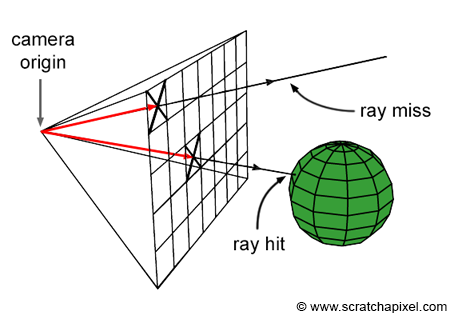
\includegraphics[width=1.0\textwidth]{secciones/imagenes/starting/gpu.png}\label{fig:marcher}
  \caption{Lanzamiento de rayos para el trazado de una escena}
\end{figure}


\section{Spheremarching\label{sec:spheremarching}}
Los algoritmos numéricos suelen ser menos costosos computacionalmente, aproximando con una variable de control que afecta al resultado trazado. En particular, se trata de una técnica reiterativa, conocidas como \textit{Raymarcher}. John C. Hart presentó en 1996 un algoritmo de esta categoría, con el nombre de  \enquote{\textit{Spheremarching}}\cite{hart1996sphere}.\\\\
Esta técnica hace uso las \textit{funciones de distancia con signo} como escena y recibe el atributo de iterativo, ya que, desde la posición de la \textit{cámara} u \textit{ojo}, incrementa el vector director hacia el pixel, conocido como \enquote{rayo} y es proporcional a la \textit{función de distancia con signo} devuelto por el vector iterado. Recibe el prefijo \enquote{\textit{Sphere}\textendash}, ya que, podemos generar, para cada iteracion, una esfera de radio igual al valor de la distancia con signo, sin ningún punto en su interior. Definimos el vector \enquote{rayo} en la iteració n-ésima, como:
\[ \Vec{p}_{n}=\Vec{ojo} + \Vec{direccion} \cdot d_{n} \]
donde \(d_{n}\) es la distancia total recorrida por todas las iteraciones:
\[d_{n}=d_{n-1} + f(\Vec{p}_{n-1})\text{ con } d_0=0\]
Al tratarse de un modelo iterativo, debemos describir las condiciones de parada del algoritmo, donde vamos a destacar tres:
\begin{enumerate}
    \item \textbf{Primera condición}. El algoritmo finalizará cuando estemos \enquote{sobre} la \textit{isosuperficie}. Al tratarse de un algoritmo numérico, vamos a aproximarla, utilizando una variable de control \(\epsilon\) que relajará la restricción de la definición de  \textit{isosuperficie}, haciendo \(f(\Vec{p}_n) < \epsilon\), ya que, si \(\epsilon = 0\), trataríamos de un modelo analítico.
    \item \textbf{Segunda condición}. Superar una cierta distancia recorrida, \(d_{n}\ge MAXIMO\), creando una esfera de trazado sobre el punto de la cámara.
    \item \textbf{Tercera condición}. Superar el número de iteraciones máximas, \(n \ge PASOS\).
\end{enumerate}
Este algoritmo devolverá \(d_n\) para el número de iteraciones fijadas, \enquote{PASOS}. Cuando el algoritmo finaliza debido a la \textbf{segunda o tercera condición}, devolverá, \(d_n=MAXIMO\), recibiendo el nombre de \enquote{\textit{fallo}}. Un fallo, representando un pixel vacío, sin superficie trazada, pudiéndose considerar el fondo de la escena.
 \begin{figure}[H]
  \centering
  \captionsetup{justification=centering}%,margin=2cm
  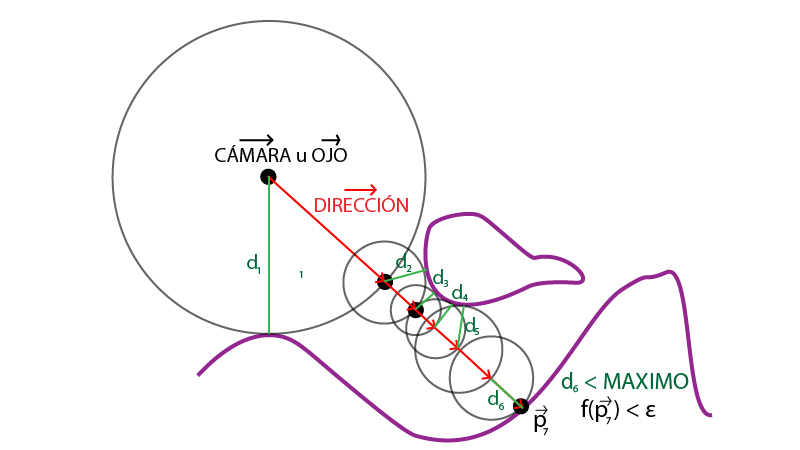
\includegraphics[width=1.0\textwidth]{secciones/imagenes/starting/spheremarching.png}\label{fig:spheremarcher}
  \caption{Ejemplo del algoritmo \textit{Spheremarching}}
\end{figure}

\newpage
\begin{lstlisting}
#define PASOS 128 // Número Máximo de Iteraciones.
#define EPSILON 0.001
#define MAXIMO 20.0 // Distancia del Plano Trasero.

// Pasamos el origen del ojo y la dirección, nos devuelve la distancia al objeto más cercano del ojo en dicha dirección.
float SphereMarching(
    in vec3 ojo, 
    in vec3 direccion
){
    float distancia = 0.0;
    // Realizamos "PASOS" iteraciones de marching.
    for(int i = 0; i < PASOS; ++i){
        // Calculamos el vector (rayo).
        vec3 rayo = ojo + direccion * distancia;
        // Aproximamos el radio de la esfera más próxima a una isosuperficie
        float radio = escena_sdf(rayo);
        // Si el radio (distancia mínima a la isosuperficie), es muy pequeña, podemos decir que estamos sobre la distancia y devolvemos el módulo del rayo.
        if(radio < EPSILON){
            return distancia;
        }
        // Incrementamos la distancia recorrida si no estamos cerca de la isosuperficie.
        distancia += radio;
        // Comprobamos que no se haya superado la distancia de dibujado máximo. Podemos considerarlos el fondo de la escena.
        if(distancia >= MAXIMO) break;
        return MAXIMO;
    }
}
\end{lstlisting}
\newpage
Este algoritmo es implementado en un \textit{shader}, aplicado para cada pixel de nuestra pantalla. En el caso  de que el algoritmo no devuelva \enquote{fallo}, podremos calcular a partir del valor devuelto \(d_n<MAXIMO\) el punto aproximado sobre la superficie, tal que:
\[ \Vec{p} = \Vec{ojo} + d_n \cdot  \Vec{direccion} \]
Conociendo los puntos de una superficie, podremos añadir información a la escena, como por ejemplo, un modelo de iluminación o materiales y texturas.\\\\
En \textit{Shadertoy}, crearemos un nuevo \textit{shader} donde se nos ofrecerá un entorno para trabajar y un código de ejemplo:
\begin{lstlisting}
void mainImage( out vec4 fragColor, in vec2 fragCoord )
{
    // Normalized pixel coordinates (from 0 to 1)
    vec2 uv = fragCoord/iResolution.xy;

    // Time varying pixel color
    vec3 col = 0.5 + 0.5*cos(iTime+uv.xyx+vec3(0,2,4));

    // Output to screen
    fragColor = vec4(col,1.0);
}
\end{lstlisting}
Observamos en el código tres variables enlazadas\ref{sec:enlaces} importante:
\begin{enumerate}
    \item \textbf{out vec4 \textit{fragColor}}. Enlaza la variable con el valor del pixel, una 4-upla, \textit{rgba}, cuyas componentes están en el intervalo \([0,1]\).
    \item \textbf{in vec2 \textit{fragCoord}}. Contiene la posición de la coordenada del pixel en pantalla, donde la primera componente representa la coordenada \(x\) y la segunda, la \(y\).
    \item \textbf{uniform vec2 \textit{iResolution}}. Se trata de una variable global que contiene información de las dimensiones en píxeles del \textit{viewport}, su primera componente, el ancho y su segunda, el alto.
\end{enumerate}
Vamos a modificar el ejemplo anterior: Situraremos la pantalla en la escena, posicionandola centrada en las coordenadas \((0,0,0)\) y preservando la relación de aspecto.  Asignaremos la posición de la cámara u ojo y calcularemos la dirección del ojo al pixel como dirección del rayo. Aplicaremos el algoritmo \textit{spheremarching} desde el ojo en la dirección calculada, en caso de devolver un fallo, utilizaremos el color negro, por el contrario, el blanco.
\newpage
\begin{lstlisting}
void mainImage(
    out vec4 fragColor, 
    in vec2 fragCoord
){
    // Normalizamos las coordendas y las reescalamos para mantener el ratio de aspecto. Transladamos al centro de la pantalla.
    vec2 uv = (fragCoord - iResolution.xy*.5) / min(iResolution.y, iResolution.x);
    // Definimos el ojo y la pantalla, que se encuentra en nuestra escena.
    vec3 ojo = vec3(0.0, 0.0, -1.0);
    vec3 pantalla = vec3(uv, 0.0);
    // La dirección del rayo es el vector normalizado que apunta desde el ojo hasta la pantalla (píxel).
    vec3 direccion = normalize(pantalla-ojo);
    // Con esto, ya podemos utilizar nuestro Sphere marcher.
    float distancia = SphereMarching(ojo, direccion);
    // El marcher nos ha devuelto una distancia inferior al plano trasero, estamos sobre la isosuperficie.
    if(distancia < MAXIMO){
        // Estamos aproximadamente sobre la isosuperficie.
        // La posición aproximada es la siguiente.
        vec3 p = ojo + direccion * distancia;
        // Utilizamos el color blanco para dibujar la isosuperficie.
        fragColor = vec4(1.0);
    }else{ // El marcher ha fallado.
        // El color negro para pintar el fondo.
        fragColor = vec4(vec3(0.0), 1.0);
    }
}
\end{lstlisting}
\newpage
La función \textit{escena\_sdf}, que se encuentra dentro de la función \textit{SphereMarching}, contiene la escena como una \textit{función de distancia con signo}. Veremos en el sexto capítulo\ref{ch:fds}, como crear nuestras escenas. Aunque, para probar nuestro algoritmo, vamos a definir una escena muy simple:
\begin{lstlisting}
/* 
Una esfera en el la coordenada (0,0,0) de radio 0.2 unidades.
*/
float escena_sdf(vec3 p){
    return length(p - vec3(0.0)) - 0.2;
}
\end{lstlisting}
Demos una pincelada de como se ha definido esta función, se calcula el módulo del punto \(\Vec{p}\), esto define una \textit{Función de Distancia} y cuya isosuperficie es únicamente un punto, \(S=\{(0,0,0)\}\), si a cada punto, restáramos \(r\) al la distancia, creamos una isosuperficie esférica de radio \(r\). Ya que, aquellos puntos cuya distancias valen \(r\), acabarán anulándose y definiendo una \textit{función de distancia con signo}.
\[S=\{\Vec{q} \in \mathbb{R}^3 / SDFEsfera_r(\Vec{q})=0\}\]
\[ SDFEsfera_r(\Vec{p})=\vert\vert\Vec{p}\vert\vert - r  \]
\begin{figure}[H]
  \centering
  \captionsetup{justification=centering}%,margin=2cm
  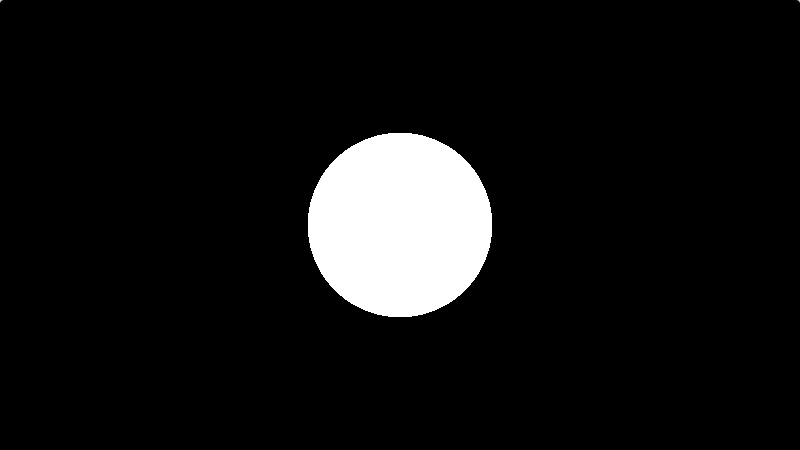
\includegraphics[width=1.0\textwidth]{secciones/imagenes/starting/sdf1.png}\label{fig:hello}
  \caption{"Hola mundo" del algoritmo \textit{SDF}.}
\end{figure}

Enlace del ejemplo \url{https://www.shadertoy.com/view/wtsfDn}\\\\
Al solo utilizar dos colores, blanco y negro, no tenemos sensación de profundidad, esto se conseguirá definiendo un modelo de iluminación.